\subsection{Robust optimization comparator}\label{sec:robust}

Table~\ref{tab:robust} compares the robust plans with the screened procedures on the 45 development instances with 20, 50 and 100 customers, and Fig.~\ref{fig:robust} shows the trade-off between service and distance; the appendix lists every setting. Every distance, including those of the OR-Tools and HGS plans, is given relative to the nominal plan found by the robust search with $\Gamma=0$; the OR-Tools nominal plans are 1.7\% longer on average.

\begin{table}[htbp]
\centering
\footnotesize
\caption{Robust comparator on the 45 development instances (exploratory): number of instances with a plan, mean validated service-event probability (\%) by size and pooled, mean distance relative to the nominal plan of the robust search ($\Gamma=0$) and mean vehicles, both over instances with a plan. A missing plan scores zero. Relief denotes the robust model with reachability relief.}
\label{tab:robust}
\begin{tabular}{@{}>{\raggedright\arraybackslash}p{4.6cm}rrrrrrr@{}}
\toprule
Configuration & Plans & $n=20$ & $n=50$ & $n=100$ & Pooled & Dist. (\%) & Veh.\\
\midrule
Conservative speed (OR-Tools) & 39 & 57.8 & 51.1 & 57.2 & 55.5 & 4.8 & 6.56\\
Capped procedure (OR-Tools) & 45 & 81.6 & 80.1 & 97.5 & 84.6 & 9.3 & 6.76\\
Capped procedure, conservative fallback (HGS) & 45 & 90.5 & 94.8 & 98.0 & 93.6 & 12.5 & 7.11\\
Robust, box, $\theta=0.4$ & 37 & 90.3 & 72.5 & 47.9 & 75.0 & 7.0 & 6.54\\
Robust, box, $\theta=0.6$ & 29 & 93.0 & 46.1 & 29.9 & 63.3 & 10.8 & 6.59\\
Relief, $\Gamma=3$, $\theta=0.4$ & 45 & 89.2 & 87.5 & 92.5 & 89.4 & 7.1 & 7.18\\
Relief, box, $\theta=0.4$ & 45 & 90.3 & 90.0 & 95.7 & 91.4 & 7.6 & 7.31\\
Relief, $\Gamma=3$, $\theta=0.6$ & 45 & 97.6 & 97.5 & 98.7 & 97.8 & 11.4 & 7.78\\
Relief, box, $\theta=0.6$ & 45 & 97.8 & 98.4 & 99.4 & 98.4 & 12.4 & 8.04\\
Screened robust & 45 & 97.0 & 82.8 & 75.1 & 87.4 & 7.9 & 7.20\\
Screened robust with relief & 45 & 97.2 & 97.4 & 97.2 & 97.2 & 10.4 & 7.64\\
\bottomrule
\end{tabular}
\end{table}

The standard robust model fails on the larger instances. Under box uncertainty it has no robust plan on 8 of the 45 instances with $\theta=0.4$ and on 16 with $\theta=0.6$. These are exactly the instances on which some customer cannot be served on time even by a direct trip at its upper travel time, so no fleet size helps. Every smaller budget $\Gamma$ failed on exactly the same instances. This is the reachability obstruction that capped contraction addresses (Section~\ref{sec:capping}). The mildest box setting, $\theta=0.2$, the robust counterpart of conservative speed, still had no plan on 4 instances and pooled 60.4\%.

Reachability relief removes the obstruction. Every relieved setting has a plan on all 45 instances, and under box uncertainty with $\theta=0.4$ relief raised pooled service by 16.4 points (Table~\ref{tab:robust-contrasts}). On the 37 instances where the standard model had a plan, the two models returned the same routes, so the whole gain comes from the instances without a standard robust plan. The relieved robust plans then compete with the screened procedures. With $\Gamma=3$ and $\theta=0.4$ they exceeded the OR-Tools capped procedure by 4.8 points on average, with an interval from $-$1.4 to 11.6, and used 0.42 more vehicles per instance. Against the HGS capped procedure the protection level decides the comparison. With $\Gamma=3$, the $\theta=0.4$ setting was 4.2 points less reliable (interval $-$7.2 to $-$0.7), with 4.6\% less distance and 0.07 more vehicles, while the $\theta=0.6$ setting was 4.2 points more reliable (interval 1.3 to 7.7) and used 0.67 more vehicles.

\begin{table}[htbp]
\centering
\footnotesize
\caption{Paired contrasts on the 45 development instances (exploratory). Service differences are in percentage points over all instances; distance differences are percentage changes and vehicle differences are means, both over instances where both configurations have a plan. Intervals are 95\% paired bootstrap intervals over instances.}
\label{tab:robust-contrasts}
\begin{tabular}{@{}>{\raggedright\arraybackslash}p{5.6cm}lll@{}}
\toprule
Contrast & Service [95\%] & Distance (\%) [95\%] & Vehicles\\
\midrule
Relief minus standard, box, $\theta=0.4$ & 16.4 [6.3, 27.1] & 0.0 [0.0, 0.0] & 0.00\\
Relief, $\Gamma=3$, $\theta=0.4$, minus OR-Tools capped procedure & 4.8 [$-$1.4, 11.6] & $-$1.7 [$-$3.4, 0.1] & 0.42\\
Relief, $\Gamma=3$, $\theta=0.4$, minus HGS capped procedure & $-$4.2 [$-$7.2, $-$0.7] & $-$4.6 [$-$6.0, $-$3.1] & 0.07\\
Relief, $\Gamma=3$, $\theta=0.6$, minus HGS capped procedure & 4.2 [1.3, 7.7] & $-$0.8 [$-$2.2, 0.8] & 0.67\\
Screened robust with relief minus HGS capped procedure & 3.6 [0.6, 7.1] & $-$1.6 [$-$3.0, $-$0.2] & 0.53\\
Screened robust with relief minus relief, box, $\theta=0.6$ & $-$1.1 [$-$1.5, $-$0.8] & $-$1.8 [$-$2.3, $-$1.2] & $-$0.40\\
\bottomrule
\end{tabular}
\end{table}

The screening layer can also wrap the robust generator. Screened robust with relief was admitted by screening on 44 of 45 instances and pooled 97.2\%, 3.6 points above the HGS capped procedure (interval 0.6 to 7.1), with 0.53 more vehicles. Against the most protective relieved setting it gave up 1.1 points and saved 1.8\% of distance, because it selects the shortest plan that passes the screen. Without relief, screening admitted a robust plan on 29 instances and pooled 87.4\%.

This comparison is exploratory. It uses the development instances, the grid was fixed before the runs, and the configurations in Table~\ref{tab:robust} are highlighted from that grid, which is reported in full. The robust plans minimize distance alone, without the slack, duration and fleet terms of the screened procedures, so differences in vehicles are part of the comparison.

\begin{figure}[ht]
 \centering
 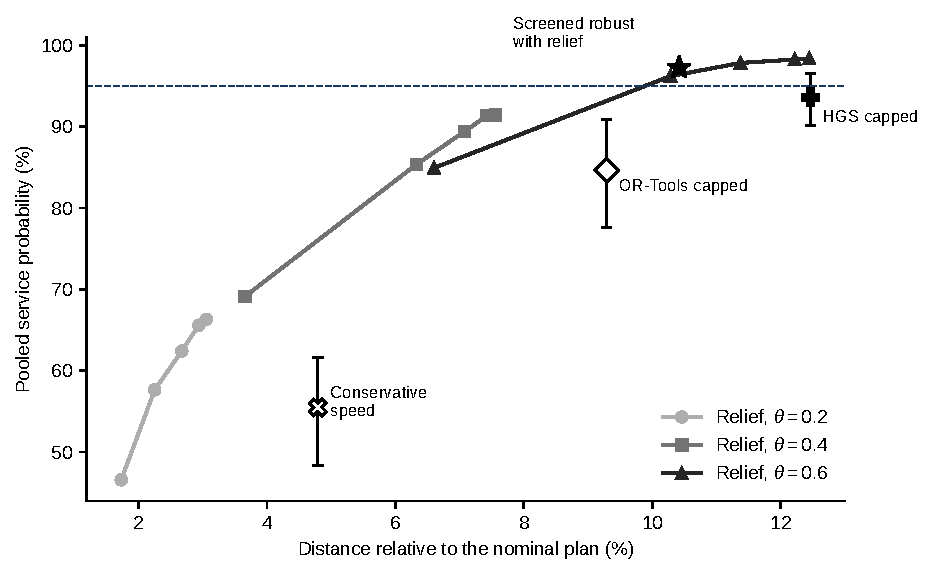
\includegraphics[width=0.93\textwidth]{Fig2.pdf}
 \caption{Pooled validated service-event probability against mean distance relative to the nominal plan of the robust search, on the 45 development instances. Lines join the relieved robust settings for each $\theta$, from $\Gamma=1$ to box uncertainty. The screened procedures (OR-Tools, HGS), screened robust with relief and conservative speed are shown separately. The dashed line marks the 95\% target}
 \label{fig:robust}
\end{figure}
